\chapter{التخليق: المردود والنقاوة}\label{ch:g10:synthesis-yield}

الأسبرين من أكثر الأدوية استعمالًا في العالم. وتبدأ قصته بلحاء الصفصاف، الذي
طالما مُضغ لمقاومة الألم والحمى؛ وفي القرن التاسع عشر رُدّت المادة الفعالة في
اللحاء إلى عائلة من المركبات حضّر منها الكيميائيون حمض الساليسيليك. ولأن حمض
الساليسيليك أقسى على المعدة من أن يؤخذ بجرعات كبيرة، فقد حُوّل إلى مادة ألطف،
هي حمض الأسيتيل ساليسيليك: الأسبرين. واليوم يُصنع بالأطنان في مفاعلات فولاذية،
بالتفاعل نفسه الذي يستطيع مختبر مدرسي أن يجريه في عصر يوم واحد. وصنع المادة
ليس إلا نصف العمل: فلا بد أيضًا من فصلها عن كل ما سواها في الدورق، وتنقيتها،
والتحقق منها، ووزنها لمعرفة كم حُصل فعلًا مما كان
ممكنًا.

\begin{recall}
\omterm{def:g10:chemical-species:extraction}{الاستخلاص}، \omterm{def:g10:chemical-species:distillation}{والتقطير}، \omterm{def:g10:chemical-species:tlc}{وكروماتوغرافيا الطبقة الرقيقة} \omterm{def:g10:chemical-species:retention-factor}{ومعامل الاحتجاز}؛ والجسم
الصلب النقي ينصهر عند درجة حرارة حادة معروفة
(\cref{ch:g10:chemical-species}). والمرشِّح يحجز الجسم الصلب ويمرر السائل
(\cref{ch:g3:separating-mixtures}). \omterm{def:g10:reaction-progress-table:extent}{وجدول التقدّم} يعطي أكبر كمية من \omterm{def:g7:chemical-reactions:reactant}{الناتج}
انطلاقًا من \omterm{def:g10:reaction-progress-table:limiting}{المتفاعل المحدِّد}
(\cref{ch:g10:reaction-progress-table}).
\end{recall}

\begin{omfigure}
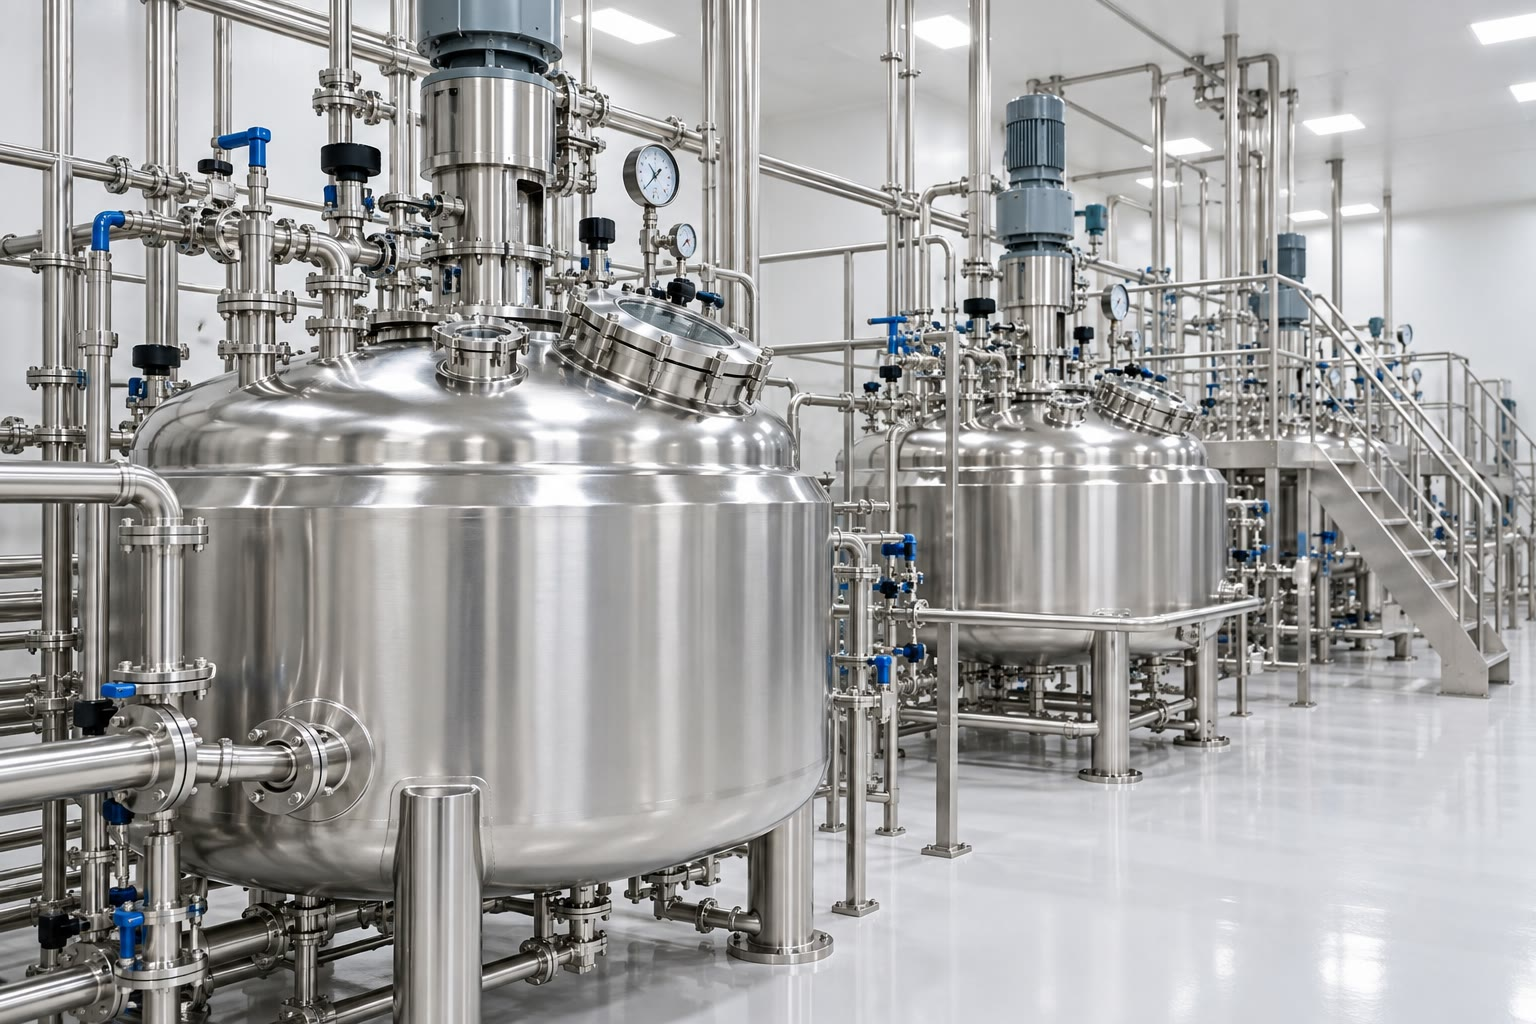
\includegraphics[width=0.55\linewidth]{images/book1/ai/g10-pharma-reactor.jpg}

{\small مفاعلات فولاذية في مصنع للأدوية: \omterm{def:g10:synthesis-yield:synthesis}{تخليق} مختبري، مكبَّر مليون
مرة.}
\end{omfigure}

\section{مراحل التخليق}

\begin{definition}[التخليق، والناتج الخام]\label{def:g10:synthesis-yield:synthesis}
\emph{التخليق}\index{تخليق} تحضير \omterm{def:g6:pure-substances-and-mixtures:species}{نوع كيميائي} \omterm{def:g7:chemical-reactions:reaction}{بتفاعل كيميائي} واحد أو أكثر،
انطلاقًا من أنواع أخرى. والجسم الصلب أو السائل المستعاد مباشرة من \omterm{def:g6:pure-substances-and-mixtures:mixture}{خليط} التفاعل،
قبل أي تنقية، هو \emph{الناتج الخام}\index{ناتج خام}: فهو لا يزال يحوي
متفاعلات ونواتج ثانوية
ومذيبًا.
\end{definition}

\begin{method}[التخطيط للتخليق]\label{met:g10:synthesis-yield:plan}
يجري \omterm{def:g10:synthesis-yield:synthesis}{التخليق} في أربع مراحل:
\begin{enumerate}
  \item \textbf{التفاعل}: اخلط \omterm{def:g7:chemical-reactions:reactant}{المتفاعلات} بالكميات المناسبة، وكثيرًا ما يكون
        أحدها بزيادة، وسخّن إن لزم.
  \item \textbf{العزل}: افصل \omterm{def:g10:synthesis-yield:synthesis}{الناتج الخام} عن \omterm{def:g6:pure-substances-and-mixtures:mixture}{خليط}
        التفاعل (\omterm{def:g3:separating-mixtures:filter}{الترشيح}، \omterm{def:g10:chemical-species:extraction}{الاستخلاص}).
  \item \textbf{التنقية}: أزل الشوائب من \omterm{def:g10:synthesis-yield:synthesis}{الناتج
        الخام} (\omterm{def:g10:synthesis-yield:recrystallisation}{إعادة التبلور} للجسم الصلب، \omterm{def:g10:chemical-species:distillation}{والتقطير}
        للسائل).
  \item \textbf{التحليل}: تحقق من هوية \omterm{def:g7:chemical-reactions:reactant}{الناتج} ونقاوته (درجة الانصهار،
        الكروماتوغرافيا)، ثم زِنه واحسب
        \omterm{def:g10:synthesis-yield:yield}{المردود}.
\end{enumerate}
\end{method}

\begin{example}[صنع الأسبرين]\label{ex:g10:synthesis-yield:aspirin}
يتفاعل حمض الساليسيليك مع أنهيدريد الإيثانويك (ويسمى أيضًا أنهيدريد الخل)
فيعطي الأسبرين وحمض الإيثانويك:
\[
  \ce{C7H6O3 + C4H6O3 -> C9H8O4 + C2H4O2}
\]
\[
  \text{حمض الإيثانويك} + \text{الأسبرين} \longleftarrow
  \text{أنهيدريد الإيثانويك} + \text{حمض الساليسيليك}.
\]
يوضع الأنهيدريد بزيادة، حتى يتفاعل حمض الساليسيليك كله؛ وحمض الإيثانويك
المتكوّن \omterm{def:g7:chemical-reactions:reactant}{ناتج} ثانوي.
\end{example}

\begin{omfigure}
\setchemfig{atom sep=1.7em}
\begin{tabular}{@{}c@{\enspace}c@{\enspace}c@{\enspace}c@{\enspace}c@{\enspace}c@{\enspace}c@{}}
\chemfig{*6(-=-(-COOH)=(-OH)-=)} & $+$ &
\chemfig{H_3C-C(=[2]O)-O-C(=[2]O)-CH_3} & $\longleftarrow$ &
\chemfig{*6(-=-(-COOH)=(-O-[:150]C(=[:90]O)-[:210]H_3C)-=)} & $+$ &
\chemfig{H_3C-C(=[2]O)-OH} \\[2pt]
\small حمض الساليسيليك & & \small أنهيدريد الإيثانويك & &
\small الأسبرين & & \small حمض الإيثانويك
\end{tabular}\par\medskip

{\small صنع الأسبرين، بالصيغ المرسومة (كل رأس من رؤوس السداسي \omterm{def:g7:atoms-and-molecules:atom}{ذرة} كربون، تحمل
\omterm{def:g7:atoms-and-molecules:atom}{ذرة} هيدروجين حيث لا يُرسم شيء آخر؛ ويشرح فصل لاحق هذا الاختصار). والمجموعة
\ce{-OH} على حلقة حمض الساليسيليك تأخذ نصف الأنهيدريد؛ ويخرج النصف الآخر
حمضَ إيثانويك.}
\end{omfigure}

\section{التسخين بالارتداد}

\begin{definition}[التسخين بالارتداد]\label{def:g10:synthesis-yield:reflux}
\emph{التسخين بالارتداد}\index{تسخين بالارتداد} تسخين \omterm{def:g6:pure-substances-and-mixtures:mixture}{خليط} تفاعل في دورق
يعلوه مكثّف رأسي: تصعد الأبخرة، وتبرد في المكثّف، ويعود السائل إلى
الدورق.
\end{definition}

\begin{proposition}[لماذا الارتداد]\label{prop:g10:synthesis-yield:why-reflux}
التسخين يسرّع معظم التفاعلات؛ والارتداد يسمح بالتسخين المدة اللازمة عند درجة
غليان \omterm{def:g6:pure-substances-and-mixtures:mixture}{الخليط} دون أن يضيع أي \omterm{def:g7:chemical-reactions:reactant}{متفاعل} أو \omterm{def:g7:chemical-reactions:reactant}{ناتج} أو \omterm{def:g6:solutions-and-solubility:solute}{مذيب} على هيئة
بخار.
\end{proposition}

\begin{proof}
لا يمكن أن ترتفع درجة حرارة سائل يغلي فوق درجة غليانه، وكل بخار يفلت من السائل
يُكثَّف ويُعاد: فلا يغادر شيء الجهاز، الذي يبقى مفتوحًا من أعلاه حتى لا يتراكم
الضغط.
\end{proof}

\begin{omfigure}
\begin{tikzpicture}[font=\small, scale=1.05]
  \pic[transform shape] at (0,0) {heatingmantle};
  \pic[transform shape] at (0,0) {rbflask={0.42}{orange!25}};
  \foreach \p in {(-0.3,0.25), (0.2,0.18), (0.45,0.4), (-0.5,0.5)}
    \fill[black!45] \p circle (0.05);
  \pic[transform shape] at (0,3.0) {condenser};
  \draw[omDef, thick, <-] (0.8,3.825) -- (1.9,3.825) node[right] {دخول الماء};
  \draw[omDef, thick, ->] (0.8,5.375) -- (1.9,5.375) node[right] {خروج الماء};
  \draw[omProp, thick, <-] (-0.18,5.8) -- (-1.4,6.1) node[left] {أعلى مفتوح};
  \draw[omProp, thick, <-] (-0.45,1.2) -- (-2.0,1.6)
    node[left, align=right] {خليط التفاعل\\ وحصى الغليان};
  \draw[omProp, thick, <-] (-1.35,-0.2) -- (-2.0,-0.6)
    node[left] {سترة التسخين};
  \draw[omThm, ->, thick] (-0.05,3.4) -- (-0.05,4.3);
  \draw[omDef, ->, thick] (0.05,4.3) -- (0.05,3.4);
  \node[omThm, anchor=east, font=\footnotesize] at (-0.45,4.6) {البخار يصعد};
  \node[omDef, anchor=west, font=\footnotesize] at (0.85,4.6) {السائل يعود نازلًا};
\end{tikzpicture}

{\small \omterm{def:g10:synthesis-yield:reflux}{التسخين بالارتداد}. يدخل الماء البارد غلاف المكثّف من الأسفل ويخرج من
الأعلى، حتى يبقى الغلاف ممتلئًا
دائمًا.}
\end{omfigure}

\begin{remark}[دخول الماء من الأسفل]\label{rem:g10:synthesis-yield:water}
لو دخل الماء من الأعلى لانحدر مباشرة إلى الأسفل وترك الجزء العلوي من الغلاف
مملوءًا \omterm{def:g4:air-a-mixture-of-gases:air}{بالهواء}؛ أما إذا دخل من الأسفل فعليه أن يملأ الغلاف كله قبل أن
يخرج.
\end{remark}

\section{العزل والتنقية}

\begin{definition}[الترشيح تحت التفريغ]\label{def:g10:synthesis-yield:vacuum-filtration}
\emph{الترشيح تحت التفريغ}\index{ترشيح تحت التفريغ} \omterm{def:g3:separating-mixtures:filter}{ترشيح} يُسحب فيه السائل
عبر ورق \omterm{def:g3:separating-mixtures:filter}{الترشيح} بالامتصاص: قمع مسطح بصفيحة مثقبة (قمع بوخنر) يوضع على دورق
ذي ذراع جانبية موصول بمضخة تفريغ.
\end{definition}

\begin{omfigure}
\begin{tikzpicture}[font=\small, scale=1.05]
  \pic[transform shape] (ff) at (0,0) {filterflask={0.12}{orange!20}};
  \fill[black!50] (-0.3,2.45) rectangle (0.3,2.8);
  \pic[transform shape] at (0,2.45) {buchner={black!8}};
  \draw[black!60, line width=2pt] (ff-arm) -- (2.6,2.2);
  \draw[omProp, thick, ->] (2.7,2.2) -- (3.4,2.2) node[right,
    align=left, text=black] {إلى\\ مضخة التفريغ};
  \draw[omProp, thick, <-] (0.7,3.8) -- (1.9,4.3) node[right, text=black]
    {بلورات على ورق الترشيح};
  \draw[omProp, thick, <-] (-0.4,0.15) -- (-1.8,0.6) node[left, text=black]
    {الراشح};
  \draw[omProp, thick, <-] (-0.3,2.6) -- (-1.8,2.9) node[left, text=black]
    {حلقة مطاطية محكمة};
\end{tikzpicture}

{\small \omterm{def:g10:synthesis-yield:vacuum-filtration}{الترشيح تحت التفريغ} بقمع بوخنر: تسحب المضخة السائل بسرعة وتترك الجسم
الصلب شبه جاف.}
\end{omfigure}

\begin{definition}[إعادة التبلور]\label{def:g10:synthesis-yield:recrystallisation}
\emph{إعادة التبلور}\index{إعادة التبلور} تنقّي جسمًا صلبًا بإذابته في أصغر حجم
ممكن من \omterm{def:g6:solutions-and-solubility:solute}{مذيب} ساخن، ثم ترك \omterm{def:g2:mixing-and-dissolving:dissolve}{المحلول} يبرد: فيتبلور \omterm{def:g7:chemical-reactions:reactant}{الناتج}، وهو أقل ذوبانًا بكثير
في البارد، بينما تبقى الشوائب، الموجودة بمقادير صغيرة،
ذائبة.
\end{definition}

\begin{method}[إعادة تبلور جسم صلب]\label{met:g10:synthesis-yield:recrystallise}
\begin{enumerate}
  \item اختر مذيبًا \omterm{def:g2:mixing-and-dissolving:dissolve}{يذوب} فيه \omterm{def:g7:chemical-reactions:reactant}{الناتج} كثيرًا وهو ساخن ولا يكاد \omterm{def:g2:mixing-and-dissolving:dissolve}{يذوب} فيه
        وهو بارد.
  \item أضف \omterm{def:g6:solutions-and-solubility:solute}{المذيب} الساخن شيئًا فشيئًا إلى الجسم الصلب الخام، حتى \omterm{def:g2:mixing-and-dissolving:dissolve}{يذوب}
        كله فقط.
  \item اترك \omterm{def:g2:mixing-and-dissolving:dissolve}{المحلول} يبرد ببطء، ثم في حمام ثلجي: فتتكوّن
        بلورات.
  \item اجمعها \omterm{def:g10:synthesis-yield:vacuum-filtration}{بالترشيح تحت التفريغ}، واغسلها بقليل من \omterm{def:g6:solutions-and-solubility:solute}{المذيب} المثلَّج،
        وجففها.
\end{enumerate}
\end{method}


\begin{omfigure}
\begin{tikzpicture}[font=\small]
  % 1. crude solid + a little hot solvent, on a hot plate
  \pic at (0,0.3) {hotplate};
  \pic at (0,0.3) {erlenmeyer={0.18}{orange!12}};
  \foreach \p in {(-0.4,0.42),(-0.15,0.38),(0.1,0.45),(0.35,0.4),(-0.3,0.55),(0.2,0.6)}
    \fill[brown!60] \p circle (0.06);
  \node[align=center, anchor=north] at (0,-0.15) {\foreignlanguage{arabic}{\babelsublr{1.} جسم صلب خام،}\\ مذيب ساخن};
  % 2. clear hot solution
  \pic at (3,0.3) {hotplate};
  \pic at (3,0.3) {erlenmeyer={0.22}{orange!12}};
  \node[align=center, anchor=north] at (3,-0.15) {\foreignlanguage{arabic}{\babelsublr{2.} ذاب كله،}\\ رائق وساخن};
  % 3. ice bath: crystals
  \fill[cyan!12, draw=black!40] (5.0,0) rectangle (7.0,1.2);
  \foreach \p in {(5.2,0.9),(6.75,1.0),(5.3,0.3),(6.8,0.25)}
    \draw[black!35, fill=white] \p ++(-0.12,-0.1) rectangle ++(0.24,0.2);
  \pic at (6,0.1) {erlenmeyer={0.2}{orange!8}};
  \foreach \x/\y in {-0.45/0.18,-0.25/0.15,0/0.2,0.25/0.15,0.45/0.2,-0.1/0.3,0.15/0.32,
                     -0.35/0.32,0.35/0.33}
    \fill[white, draw=black!55] (6+\x,0.1+\y) -- ++(0.07,0.06) -- ++(0.07,-0.06)
      -- ++(-0.07,-0.06) -- cycle;
  \node[align=center, anchor=north] at (6,-0.15) {\foreignlanguage{arabic}{\babelsublr{3.} تبريد في الثلج:}\\ تتكوّن بلورات};
  % 4. filter
  \pic at (9,0) {filterflask={0.12}{orange!12}};
  \pic at (9,2.45) {buchner={black!12}};
  \fill[black!50] (8.7,2.45) rectangle (9.3,2.8);
  \node[align=center, anchor=north] at (9,-0.15) {\foreignlanguage{arabic}{\babelsublr{4.} ترشيح تحت التفريغ،}\\ غسل بارد، تجفيف};
\end{tikzpicture}

{\small \omterm{def:g10:synthesis-yield:recrystallisation}{إعادة التبلور} في أربع خطوات. تبقى الشوائب ذائبة في \omterm{def:g6:solutions-and-solubility:solute}{المذيب} البارد
وتنتقل إلى \omterm{def:g3:separating-mixtures:filter}{الراشح}.}
\end{omfigure}

\begin{remark}[الخسائر لا مفر منها]\label{rem:g10:synthesis-yield:losses}
% ledger: sol:aspirin-25, sol:aspirin-37
حتى وهو بارد يُبقي \omterm{def:g6:solutions-and-solubility:solute}{المذيب} بعض \omterm{def:g7:chemical-reactions:reactant}{الناتج} ذائبًا. فالأسبرين \omterm{def:g2:mixing-and-dissolving:dissolve}{يذوب} في الماء بنحو
\qty{3.3}{g/L} عند \qty{25}{\celsius}، وبثلاثة أضعاف ذلك عند
\qty{37}{\celsius}، وبأكثر بكثير وهو أسخن: فكل ميليلتر من \omterm{def:g3:separating-mixtures:filter}{الراشح} ومن ماء الغسل
يحمل معه قليلًا من الأسبرين. \omterm{def:g10:synthesis-yield:recrystallisation}{فإعادة التبلور} تشتري النقاوة بثمن من
الكتلة.
\end{remark}

\section{تحليل الناتج}

\begin{proposition}[اختباران للنقاوة]\label{prop:g10:synthesis-yield:checks}
يكون الجسم الصلب المخلَّق نقيًا، في حدود هذين الاختبارين، حين:
\begin{itemize}
  \item ينصهر انصهارًا حادًا عند درجة الانصهار المذكورة في الجداول؛
  \item يعطي على صفيحة \omterm{def:g10:chemical-species:tlc}{كروماتوغرافيا الطبقة الرقيقة} بقعة واحدة،
        في ارتفاع عيّنة من \omterm{def:g6:pure-substances-and-mixtures:pure-substance}{المادة النقية} نفسه.
\end{itemize}
\end{proposition}

\begin{proof}
نقبله: فالشائبة تخفض درجة الانصهار وتمدّها على مجال
(\cref{ch:g10:chemical-species})، والنوع الثاني يقطع عادة مسافة مختلفة على
الصفيحة.
\end{proof}

\begin{omfigure}
\begin{tikzpicture}[font=\small, scale=1.3]
  \pic[transform shape] at (0,0) {tlcplate};
  \draw[black!50, dashed] (-0.7,2.7) -- (0.7,2.7);
  % lanes: C crude, R recrystallised, A aspirin, S salicylic acid
  \foreach \x/\l in {-0.5/C,-0.17/R,0.17/A,0.5/S}
    \node[font=\footnotesize, anchor=north] at (\x,0.38) {\l};
  \fill[omDef!70] (-0.5,1.75) ellipse (0.09 and 0.06);
  \fill[omDef!40] (-0.5,1.25) ellipse (0.09 and 0.06);
  \fill[omDef!70] (-0.17,1.75) ellipse (0.09 and 0.06);
  \fill[omDef!70] (0.17,1.75) ellipse (0.09 and 0.06);
  \fill[omDef!70] (0.5,1.25) ellipse (0.09 and 0.06);
  \node[anchor=west, font=\footnotesize] at (0.85,2.7) {جبهة المذيب};
  \node[anchor=west, font=\footnotesize] at (0.85,0.4) {خط الانطلاق};
\end{tikzpicture}

{\small كروماتوغرافيا \omterm{def:g10:synthesis-yield:synthesis}{الناتج الخام} (C) \omterm{def:g7:chemical-reactions:reactant}{والناتج} المعاد تبلوره (R) إلى جانب الأسبرين
النقي (A) وحمض الساليسيليك (S)، تحت الأشعة فوق البنفسجية. لا يزال \omterm{def:g10:synthesis-yield:synthesis}{الناتج الخام}
يحوي حمض الساليسيليك؛ أما \omterm{def:g7:chemical-reactions:reactant}{الناتج} المعاد تبلوره فلا.}
\end{omfigure}

\section{المردود}

\begin{definition}[المردود]\label{def:g10:synthesis-yield:yield}
\emph{المردود}\index{مردود} $\eta$ \omterm{def:g10:synthesis-yield:synthesis}{للتخليق} هو نسبة كمية \omterm{def:g7:chemical-reactions:reactant}{الناتج} المحصَّلة فعلًا،
نقيةً وجافة، إلى أكبر كمية يمكن أن يعطيها \omterm{def:g10:reaction-progress-table:limiting}{المتفاعل
المحدِّد}:
\[
  \eta = \frac{n_{\text{المحصَّلة}}}{n_{\max}} ,
\]
ويُعطى عادة بالنسبة المئوية.
\end{definition}

\begin{proposition}[المردود من الكتل]\label{prop:g10:synthesis-yield:masses}
بما أن الكميتين المحصَّلة والقصوى تخصان \omterm{def:g7:chemical-reactions:reactant}{الناتج} نفسه، وكتلته المولية
$M$، \omterm{def:g10:synthesis-yield:yield}{فالمردود} هو أيضًا نسبة الكتلتين:
\[
  \eta = \frac{m_{\text{المحصَّلة}}}{m_{\max}},
  \qquad m_{\max} = n_{\max} \times M,
\]
حيث تأتي $n_{\max}$ من \omterm{def:g10:reaction-progress-table:extent}{جدول التقدّم}، عند $x = x_{\max}$.
\end{proposition}

\begin{proof}
$m_{\text{المحصَّلة}} / m_{\max} = (n_{\text{المحصَّلة}} M) / (n_{\max} M)
= n_{\text{المحصَّلة}} / n_{\max}$.
\end{proof}

\begin{example}[مردود تخليق صغير]\label{ex:g10:synthesis-yield:small}
% ledger: aw:C, aw:H, aw:O
تتفاعل \qty{1.38}{g} من حمض الساليسيليك ($M = \qty{138.0}{g/mol}$)، أي
\qty{0.0100}{mol}، مع أنهيدريد الإيثانويك بزيادة. فأكبر كمية من الأسبرين
\qty{0.0100}{mol}، أي $0.0100 \times 180.0 = \qty{1.80}{g}$. فإذا حُصل على
\qty{1.35}{g} من الأسبرين النقي الجاف، كان $\eta = 1.35 / 1.80 = 0.75$، أي
\omterm{def:g10:synthesis-yield:yield}{مردود} قدره \qty{75}{\percent}.
\end{example}

\begin{remark}[لماذا تقل المردودات عن 100 \%]\label{rem:g10:synthesis-yield:below}
يضيع شيء من \omterm{def:g7:chemical-reactions:reactant}{الناتج} في كل مرحلة: يلتصق بالأدوات الزجاجية، \omterm{def:g2:mixing-and-dissolving:dissolve}{ويذوب} في \omterm{def:g3:separating-mixtures:filter}{الراشح} وماء
الغسل، ويبقى في \omterm{def:g10:synthesis-yield:recrystallisation}{إعادة التبلور}؛ وبعض التفاعلات تعطي أيضًا نواتج جانبية، أو تتوقف
قبل أن يُستهلك \omterm{def:g10:reaction-progress-table:limiting}{المتفاعل المحدِّد}. \omterm{def:g10:synthesis-yield:yield}{والمردود} الذي يتجاوز \qty{100}{\percent}
علامة خطأ دائمًا، وفي الغالب \omterm{def:g7:chemical-reactions:reactant}{ناتج} وُزن وهو لا يزال رطبًا أو غير نقي.
\end{remark}

\begin{inthelab}[صنع الأسبرين]
في دورق جاف يخلط المعلم حمض الساليسيليك مع زيادة من أنهيدريد الإيثانويك وبضع
قطرات من حمض يسرّع التفاعل، ويسخّن \omterm{def:g6:pure-substances-and-mixtures:mixture}{الخليط} بالارتداد في حمام مائي عند نحو
\qty{80}{\celsius} ربع ساعة. وبعد التبريد يُضاف ماء بارد: فيتفاعل معه الأنهيدريد
الزائد، ويخرج الأسبرين، القليل \omterm{def:g2:mixing-and-dissolving:dissolve}{الذوبان} في الماء البارد، بلورات بيضاء. فتُجمع
\omterm{def:g10:synthesis-yield:vacuum-filtration}{بالترشيح تحت التفريغ}، ويُعاد تبلورها، وتُجفف، وتُوزن، وتُقاس درجة
انصهارها.
\end{inthelab}

\begin{safety}{\ghs[0.82cm]{GHS02}\ghs[0.82cm]{GHS05}\ghs[0.82cm]{GHS06}\ghs[0.82cm]{GHS07}}
% ledger: ghs:acetic-anhydride, ghs:salicylic, ghs:aspirin
أنهيدريد الإيثانويك قابل للاشتعال، وضار إذا ابتُلع أو استُنشق، ويسبب حروقًا
شديدة للجلد والعينين: يتناوله المعلم تحت ساحبة الغازات، بالقفازات والنظارات
الواقية. وحمض الساليسيليك ضار إذا ابتُلع وقد يؤذي العينين. والأسبرين المصنوع في
المختبر لا يؤخذ أبدًا دواءً.
\end{safety}

\begin{omfigure}
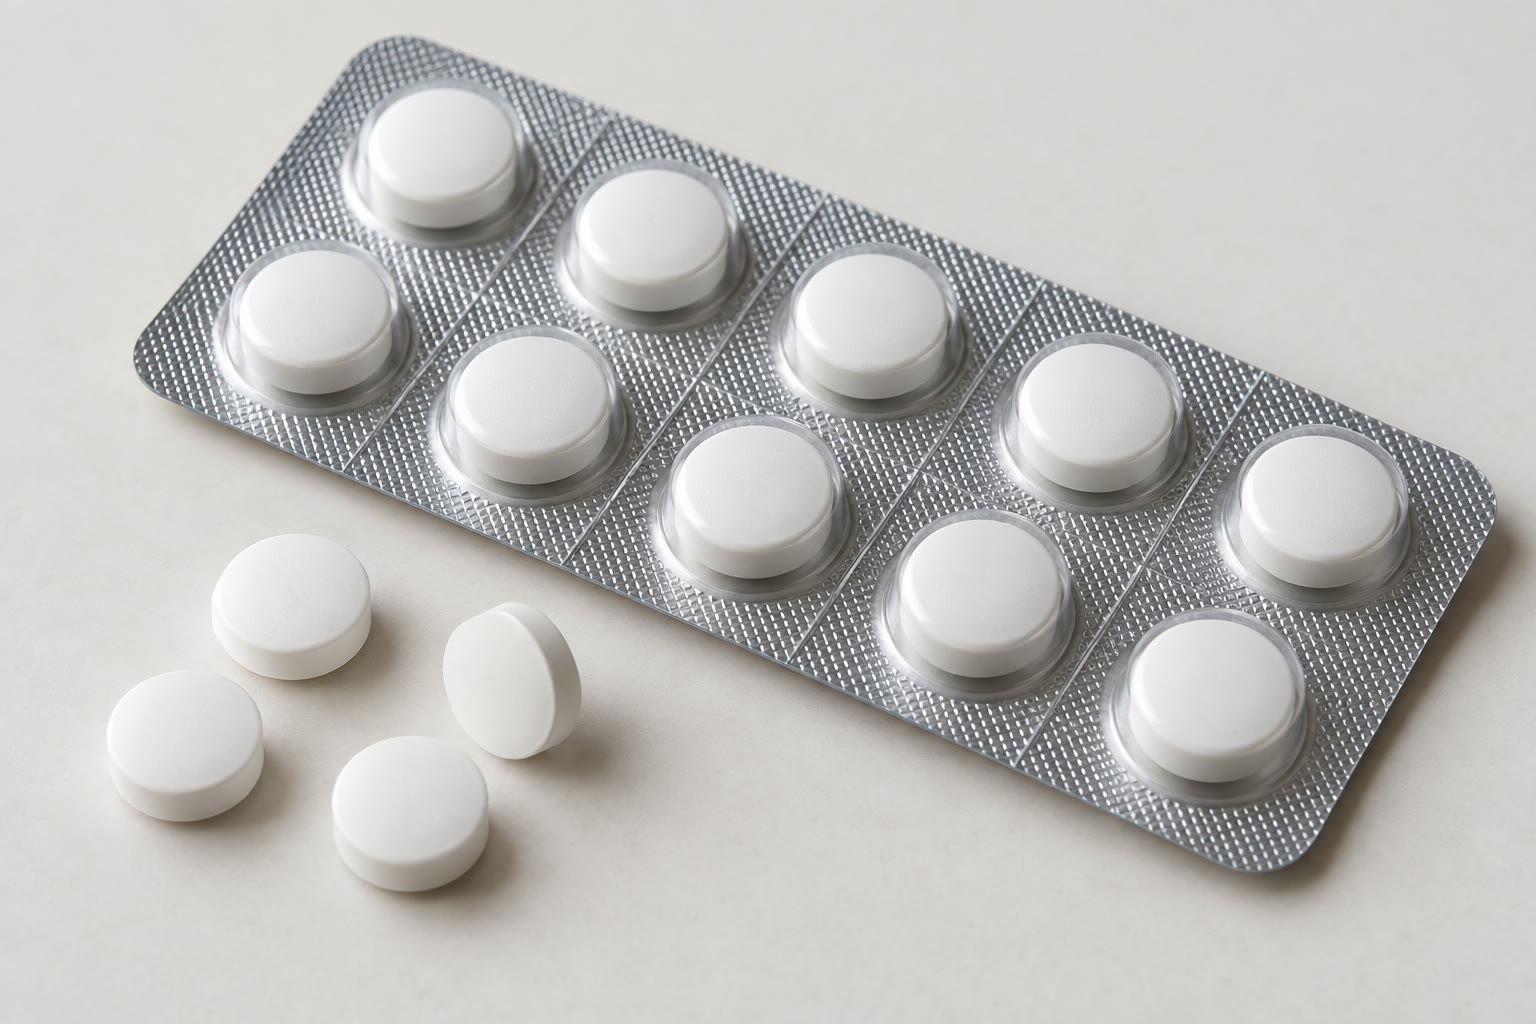
\includegraphics[width=0.45\linewidth]{images/book1/ai/g10-aspirin-tablets.jpg}

{\small أقراص الأسبرين: يحوي كل منها كتلة موزونة من \omterm{def:g6:pure-substances-and-mixtures:pure-substance}{المادة النقية}، ممزوجة
بمادة رابطة.}
\end{omfigure}

\section{تمارين}


\begin{exercise}[$\star$]\label{exo:g10:synthesis-yield:1}
كان يمكن \omterm{def:g10:synthesis-yield:synthesis}{لتخليق} أن يعطي على الأكثر \qty{5.0}{g} من \omterm{def:g7:chemical-reactions:reactant}{الناتج}؛ وحُصل على
\qty{4.2}{g} من \omterm{def:g7:chemical-reactions:reactant}{الناتج} النقي الجاف. احسب \omterm{def:g10:synthesis-yield:yield}{المردود}.
\end{exercise}

\begin{exercise}[$\star$]\label{exo:g10:synthesis-yield:2}
رتّب هذه المراحل من \omterm{def:g10:synthesis-yield:synthesis}{تخليق}: قياس درجة الانصهار؛ \omterm{def:g10:synthesis-yield:reflux}{والتسخين بالارتداد}؛ \omterm{def:g10:synthesis-yield:recrystallisation}{وإعادة
التبلور}؛ \omterm{def:g10:synthesis-yield:vacuum-filtration}{والترشيح تحت التفريغ} \omterm{def:g10:synthesis-yield:synthesis}{للناتج الخام}؛ ووزن
\omterm{def:g7:chemical-reactions:reactant}{المتفاعلات}.
\end{exercise}

\begin{exercise}[$\star$]\label{exo:g10:synthesis-yield:3}
في تركيب الارتداد، لماذا يُدخَل ماء التبريد في المكثّف من الأسفل؟ ولماذا
يُترك أعلى المكثّف مفتوحًا؟
\end{exercise}

\begin{exercise}[$\star$]\label{exo:g10:synthesis-yield:4}
ما الخاصيتان اللتان يجب أن تكونا في \omterm{def:g6:solutions-and-solubility:solute}{مذيب} لإعادة تبلور \omterm{def:g7:chemical-reactions:reactant}{ناتج}؟ وإلى أين تنتهي
الشوائب؟
\end{exercise}

\begin{exercise}[$\star$]\label{exo:g10:synthesis-yield:5}
% ledger: mp:aspirin
تنصهر عيّنة من الأسبرين المخلَّق بين \qty{124}{\celsius}
و\qty{130}{\celsius}. والأسبرين النقي ينصهر عند نحو \qty{135}{\celsius}. هل
العيّنة نقية؟ وماذا يجب أن يُفعل؟
\end{exercise}

\begin{exercise}[$\star\star$]\label{exo:g10:synthesis-yield:6}
تتفاعل \qty{2.00}{g} من حمض الساليسيليك مع أنهيدريد الإيثانويك بزيادة؛ ويُحصل
على \qty{2.03}{g} من الأسبرين النقي الجاف. احسب أكبر كتلة ممكنة من الأسبرين،
\omterm{def:g10:synthesis-yield:yield}{والمردود}.
\end{exercise}

\begin{exercise}[$\star\star$]\label{exo:g10:synthesis-yield:7}
تزن تلميذة أسبرينها وهو لا يزال رطبًا فتجد مردودًا قدره
\qty{104}{\percent}. علّل. وهل يعطي وزن \omterm{def:g10:synthesis-yield:synthesis}{الناتج الخام}، غير المنقى لكنه جاف،
مردودًا أعلى من \omterm{def:g10:synthesis-yield:yield}{المردود} الحقيقي أم أدنى منه؟
\end{exercise}

\begin{exercise}[$\star\star$]\label{exo:g10:synthesis-yield:8}
اذكر ميزتين \omterm{def:g10:synthesis-yield:vacuum-filtration}{للترشيح تحت التفريغ} على \omterm{def:g3:separating-mixtures:filter}{الترشيح} العادي عبر مخروط من الورق،
لجمع البلورات.
\end{exercise}

\begin{exercise}[$\star\star$]\label{exo:g10:synthesis-yield:9}
على صفيحة كروماتوغرافيا قطعت جبهة \omterm{def:g6:solutions-and-solubility:solute}{المذيب} \qty{5.0}{cm}. وقطعت بقعة \omterm{def:g7:chemical-reactions:reactant}{ناتج} مخلَّق
\qty{3.1}{cm}، وبقعة الأسبرين النقي \qty{3.1}{cm}، وبقعة حمض الساليسيليك
\qty{2.2}{cm}. احسب معاملات الاحتجاز الثلاثة. وماذا يمكن أن نستنتج عن
الناتج؟
\end{exercise}

\begin{exercise}[$\star\star$]\label{exo:g10:synthesis-yield:10}
\omterm{def:g6:solutions-and-solubility:solubility}{ذوبانية} \omterm{def:g7:chemical-reactions:reactant}{ناتج} في مذيبين هي:
\begin{center}
\begin{tabular}{lcc}
\hline
\omterm{def:g6:solutions-and-solubility:solute}{المذيب} & بارد (\qty{20}{\celsius}) & ساخن (قرب الغليان) \\
\hline
A & \qty{2}{g/L} & \qty{150}{g/L} \\
B & \qty{80}{g/L} & \qty{120}{g/L} \\
\hline
\end{tabular}
\end{center}
أي المذيبين أفضل \omterm{def:g10:synthesis-yield:recrystallisation}{لإعادة التبلور}؟ ولكتلة \qty{3.0}{g} من \omterm{def:g10:synthesis-yield:synthesis}{الناتج الخام}، ما حجم \omterm{def:g6:solutions-and-solubility:solute}{المذيب}
الساخن اللازم تقريبًا، وما أكبر كتلة تبقى ذائبة بعد
التبريد؟
\end{exercise}

\begin{exercise}[$\star\star$]\label{exo:g10:synthesis-yield:11}
لماذا لا يُملأ الدورق الكروي في تركيب الارتداد أبدًا أكثر من نصفه؟ ولماذا
يُضاف حصى الغليان؟
\end{exercise}

\begin{exercise}[$\star\star\star$]\label{exo:g10:synthesis-yield:12}
يُصنع دواء في مرحلتين، مردوداهما \qty{80}{\percent}
و\qty{70}{\percent}. ما \omterm{def:g10:synthesis-yield:yield}{المردود} الكلي؟ وكم يكون لثلاث مراحل \omterm{def:g10:synthesis-yield:yield}{مردود} كل منها
\qty{90}{\percent}؟ ولماذا يحاول الكيميائيون صنع الأدوية في أقل عدد ممكن من
المراحل؟
\end{exercise}

\begin{exercise}[$\star\star\star$]\label{exo:g10:synthesis-yield:13}
% ledger: sol:aspirin-25
\omterm{def:g2:mixing-and-dissolving:dissolve}{يذوب} الأسبرين في الماء بنحو \qty{3.3}{g/L} عند
\qty{25}{\celsius}. تُغسل البلورات بحجم \qty{50}{mL} من الماء في هذه الدرجة.
ما كتلة الأسبرين التي قد تضيع على الأكثر؟ ولماذا يُبرَّد ماء الغسل في الثلج
أولًا؟
\end{exercise}

\begin{exercise}[$\star\star\star$]\label{exo:g10:synthesis-yield:14}
تُخلط \qty{2.76}{g} من حمض الساليسيليك مع \qty{0.0500}{mol} من
أنهيدريد الإيثانويك. وبعد التفاعل يُضاف ماء يُتلف الأنهيدريد
الزائد: \ce{C4H6O3 + H2O -> 2C2H4O2}.
\begin{enumerate}
  \item املأ جدول تقدّم \omterm{def:g10:synthesis-yield:synthesis}{التخليق}؛ ما كمية الأنهيدريد
        المتبقية؟
  \item ما الكمية الكلية لحمض الإيثانويك الموجودة في النهاية؟
\end{enumerate}
\end{exercise}

\begin{exercise}[$\star\star\star$]\label{exo:g10:synthesis-yield:15}
على مصنع أن يصنع \qty{1.00}{t} من الأسبرين، \omterm{def:g10:synthesis-yield:yield}{بمردود} كلي قدره
\qty{85}{\percent} انطلاقًا من حمض الساليسيليك. ما كتلة حمض الساليسيليك التي
يجب أن يشتريها؟
\end{exercise}

\section{مسألة: صنع الأسبرين}

\begin{problem}[{مسألة نهاية الأسبوع --- من ثلاثة غرامات من حمض الساليسيليك إلى
مرطبان من الأسبرين النقي: ما المردود؟}]
\label{pb:g10:synthesis-yield:1}
% ledger: rho:acetic-anhydride, mp:aspirin, mp:salicylic, sol:aspirin-25, aw:C, aw:H, aw:O
يصنع صف الأسبرين. في الدورق: \qty{3.0}{g} من حمض الساليسيليك
و\qty{6.0}{mL} من أنهيدريد الإيثانويك، كثافته \qty{1.08}{g/mL}، مع بضع
قطرات من حمض؛ ويُسخَّن \omterm{def:g6:pure-substances-and-mixtures:mixture}{الخليط} بالارتداد. \omterm{def:g10:synthesis-yield:synthesis}{والناتج الخام} المجموع \omterm{def:g10:synthesis-yield:vacuum-filtration}{بالترشيح تحت
التفريغ} يزن \qty{3.6}{g} وهو رطب و\qty{3.3}{g} بعد التجفيف. وبعد \omterm{def:g10:synthesis-yield:recrystallisation}{إعادة
التبلور} والتجفيف يبقى \qty{2.7}{g} من البلورات
البيضاء.

\medskip
\noindent\textbf{الجزء الأول --- التفاعل.}
\begin{enumerate}
  \item تحقق من أن المعادلة
        \ce{C7H6O3 + C4H6O3 -> C9H8O4 + C2H4O2} موزونة.
  \item احسب الكتل المولية لحمض الساليسيليك وأنهيدريد الإيثانويك
        والأسبرين وحمض الإيثانويك.
  \item سمِّ \omterm{def:g7:chemical-reactions:reactant}{المتفاعلات}، \omterm{def:g7:chemical-reactions:reactant}{والناتج} المطلوب، \omterm{def:g7:chemical-reactions:reactant}{والناتج} الثانوي.
  \item لماذا يُسخَّن \omterm{def:g6:pure-substances-and-mixtures:mixture}{الخليط} بالارتداد لا في دورق
        مفتوح؟
\end{enumerate}

\medskip
\noindent\textbf{الجزء الثاني --- أكبر كتلة ممكنة.}
\begin{enumerate}[resume]
  \item احسب الكمية الابتدائية لحمض الساليسيليك.
  \item احسب كتلة أنهيدريد الإيثانويك، ثم كميته.
  \item املأ \omterm{def:g10:reaction-progress-table:extent}{جدول التقدّم}. أي المتفاعلين محدِّد؟ أعطِ
        $x_{\max}$.
  \item استنتج أكبر كتلة ممكنة من الأسبرين.
  \item لماذا يوضع الأنهيدريد، لا حمض الساليسيليك،
        بزيادة؟
\end{enumerate}

\medskip
\noindent\textbf{الجزء الثالث --- العزل والتنقية.}
\begin{enumerate}[resume]
  \item لماذا لا يمكن استعمال الكتلة الرطبة، \qty{3.6}{g}، لحساب
        \omterm{def:g10:synthesis-yield:yield}{مردود}؟
  \item احسب \omterm{def:g10:synthesis-yield:yield}{مردود} \omterm{def:g10:synthesis-yield:synthesis}{الناتج الخام} الجاف.
  \item لماذا تُنقص \omterm{def:g10:synthesis-yield:recrystallisation}{إعادة التبلور} الكتلة؟
  \item غُسلت البلورات بحجم \qty{30}{mL} من الماء عند
        \qty{25}{\celsius}، حيث \omterm{def:g2:mixing-and-dissolving:dissolve}{يذوب} الأسبرين بنحو
        \qty{3.3}{g/L}. ما أكبر كتلة قد تضيع بهذه الطريقة؟
  \item احسب \omterm{def:g10:synthesis-yield:yield}{مردود} \omterm{def:g7:chemical-reactions:reactant}{الناتج} النقي.
\end{enumerate}

\medskip
\noindent\textbf{الجزء الرابع --- التحقق من \omterm{def:g7:chemical-reactions:reactant}{الناتج}.}
\begin{enumerate}[resume]
  \item تنصهر البلورات المعاد تبلورها انصهارًا حادًا عند \qty{135}{\celsius}.
        ماذا يبيّن ذلك؟
  \item انصهر \omterm{def:g10:synthesis-yield:synthesis}{الناتج الخام} بين \qty{120}{\celsius}
        و\qty{131}{\celsius}. ماذا يبيّن ذلك؟
  \item على صفيحة كروماتوغرافيا يعطي \omterm{def:g10:synthesis-yield:synthesis}{الناتج الخام} بقعتين،
        إحداهما في ارتفاع الأسبرين النقي والأخرى في ارتفاع
        حمض الساليسيليك؛ ويعطي \omterm{def:g7:chemical-reactions:reactant}{الناتج} المعاد تبلوره بقعة واحدة، في
        ارتفاع الأسبرين. استنتج.
  \item قطعت بقعة \omterm{def:g7:chemical-reactions:reactant}{الناتج} المعاد تبلوره \qty{3.1}{cm} وقطعت
        جبهة \omterm{def:g6:solutions-and-solubility:solute}{المذيب} \qty{5.0}{cm}. احسب معامل احتجازه.
  \item بين التفاعل \omterm{def:g10:synthesis-yield:recrystallisation}{وإعادة التبلور}، أي جزء من العمل أضاع
        من الأسبرين أكثر؟
  \item اذكر الجواب النهائي: ما \omterm{def:g10:synthesis-yield:yield}{مردود} \omterm{def:g10:synthesis-yield:synthesis}{التخليق}؟
\end{enumerate}
\end{problem}
